\chapter{Расширяющаяся ньютоновская Вселенная}

\lectureoverview{Современная космология начинается тогда, когда сама Вселенная рассматривается как физическая система. Исходя из крупномасштабных изотропии и однородности, мы вводим сопутствующую сетку и описываем её движение с помощью единственного масштабного множителя \(a(t)\). Затем теорема Ньютона о сферической оболочке сводит гравитационную многочастичную задачу к уравнению для \(a(t)\). Закон сохранения энергии различает повторно коллапсирующие, критические и вечно расширяющиеся вселенные, а критический случай с доминированием вещества даёт первое уравнение Фридмана и закон \(a(t)\propto t^{2/3}\).}

\section{Когда космология стала физикой}

Космология как предмет стара, но количественная космология молода. Для нашей цели нет нужды начинать с греков. Полезными историческими отправными точками являются открытие Хабблом космического расширения во второй четверти двадцатого века и, позднее, понимание того, что микроволновый фон с температурой около трёх кельвинов представляет собой остаток горячей ранней Вселенной.

Прежде чем измерения стали точными, значительная часть астрономии по необходимости напоминала естественную историю. Обнаруживали необычную звезду, классифицировали своеобразную галактику, измеряли всё, что удавалось измерить, и составляли каталог объектов. Эти объекты, разумеется, были физическими системами: они обладали угловым моментом, содержали химические элементы и подчинялись механике. Решающий сдвиг состоял в том, чтобы рассматривать \emph{всю Вселенную} как одну физическую систему, описываемую уравнениями, достаточно точными для сопоставления с наблюдениями.

Именно это здесь и является предметом. Мы не будем просто перечислять содержимое Вселенной; мы будем спрашивать, каковы её переменные, её движение и её динамический закон. Уравнения — не украшение, добавляемое к космологии задним числом. Именно с их помощью Вселенная становится задачей физики.

Исторически расширяющаяся Вселенная была понята на языке общей теории относительности. Однако логически значительная часть первого рассуждения ньютоновская. Физик XVII века, угадавший правильное крупномасштабное движение, мог бы вывести удивительно хорошую модель. Смысл начала с Ньютона не в том, чтобы заменить теорию относительности, а в том, чтобы выявить механику, которую она позднее геометрически переформулирует.

\section{Изотропия, однородность и космологический принцип}

Первый шаг здесь — наблюдательный. На достаточно больших масштабах Вселенная приблизительно \emph{изотропна}: после усреднения по участкам неба и если смотреть за пределы переднего плана Млечного Пути, она выглядит почти одинаково во всех направлениях. Это не утверждение о точной равномерности. Смотреть прямо на близкую звезду — не то же самое, что смотреть в пустой участок неба, и распределение вещества содержит реальную структуру. Изотропия — это усреднённое крупномасштабное утверждение.

Однородность — другое утверждение. Оно говорит, что усреднённая Вселенная одинакова от места к месту. Наблюдатель, отстоящий от нас на много галактик, должен после того же крупномасштабного усреднения видеть примерно тот же тип Вселенной, что и мы.

В первом приближении галактику можно рассматривать просто как материальную точку. Наблюдаемая Вселенная содержит примерно
\begin{equation}
N_{\rm gal}\sim 10^{11}
\end{equation}
галактик, в каждой порядка \(10^{11}\) звёзд. Это даёт приблизительно \(10^{22}\) звёзд. Если взять 10 планет на звезду как заведомо грубую оценку по порядку величины, получится \(10^{23}\) планет — забавно близко к молю планет. Эта численная оценка не является частью динамики, но она фиксирует масштаб идеализируемой системы.

\begin{classroomqa}
\classquestion{Сколько галактик содержится в наблюдаемой Вселенной по порядку величины?}
\lecturerresponse{Около ста миллиардов, то есть \(10^{11}\). При примерно \(10^{11}\) звёздах на галактику это означает приблизительно \(10^{22}\) звёзд в видимой Вселенной. Эти оценки масштаба полезно держать в уме, хотя в последующем вычислении каждая галактика заменяется одной материальной точкой. \lecturetimestamp{00:06:08--00:07:05}}
\end{classroomqa}

Почему изотропия вокруг нас должна наводить на мысль об однородности? Представим изотропное распределение, которое \emph{не} является однородным. Его плотность должна была бы меняться с расстоянием до нас, оставаясь независимой от направления: фактически это был бы рисунок концентрических оболочек вокруг нашего положения. Наблюдатель, смещённый относительно общего центра, уже не увидел бы изотропии. Таким образом, есть две возможности:
\begin{enumerate}
\item мы занимаем выделенный центр, вокруг которого устроена Вселенная; или
\item крупномасштабное распределение приблизительно однородно, так что ни одна занятая точка не выделена.
\end{enumerate}
Вторая возможность экономнее. Изотропия вместе с отказом приписывать себе привилегированное космическое положение приводит к однородности.

\begin{classroomqa}
\classquestion{Какую форму могло бы принять изотропное, но неоднородное распределение?}
\lecturerresponse{Его изменение могло бы зависеть только от расстояния до нас, создавая оболочечную картину с центром в нашем положении. Стоит сместить наблюдателя от этого центра, и картина перестаёт быть изотропной. Если только наше местоположение не является особым, изотропия, следовательно, указывает на однородность. \lecturetimestamp{00:07:06--00:08:54}}
\end{classroomqa}

Это объединённое предположение называется \emph{космологическим принципом}: на достаточно больших масштабах Вселенная пространственно однородна и изотропна. Называя это принципом, мы тем самым ничего не доказываем. Исторически космологи приняли это предположение раньше, чем наблюдения дали ему серьёзное обоснование. Его статус определяется эмпирическим успехом.

Но и однородность не является точной. Галактики образуют скопления и сверхскопления, и давно ведутся обсуждения структур, простирающихся на очень большие доли видимого неба. Корректное утверждение состоит в том, что флуктуации усредняются, когда область усреднения достаточно велика---в этом вводном обсуждении порядка сотен миллионов и вплоть до примерно миллиарда световых лет. Этот масштаб может быть уточнён наблюдениями; метод состоит в том, чтобы переходить к крупнозернистому усреднению, пока локальная структура не перестанет доминировать в описании.

\begin{classroomqa}
\audiencequestion{Даёт ли равномерность космического микроволнового фона свидетельство в пользу космологического принципа?}
\lecturerresponse{Да. Космологический принцип был предложен ещё до того, как появились сильные наблюдательные основания в его пользу, но микроволновый фон позднее показал, что первичная Вселенная была чрезвычайно гладкой. Галактики и скопления выросли из малых отклонений от этого гладкого состояния; они не стирают крупномасштабных свидетельств в его пользу. \lecturetimestamp{00:10:53--00:11:43}}
\end{classroomqa}

\section{Сетка, движущаяся вместе с галактиками}

Как только выбрано наблюдательное приближение, надо выбрать переменные. Один ответ, который дают в аудитории на вопрос «Каков первый шаг при постановке физической задачи?», состоит в том, что нужно знать переменные; традиционный ответ — наточить карандаш. Здесь важная переменная находится благодаря удачному выбору координат.

Представьте трёхмерную сетку с метками \(x,y,z\). Эти метки не обязаны быть расстояниями, измеренными в метрах. Это координатные числа. Выберем сетку так, чтобы после усреднения малых пекулярных движений каждая галактика оставалась в фиксированной точке сетки. Тогда галактики оказываются \emph{сопутствующими}.

Такой выбор был бы бесполезен, если бы галактики двигались случайно. Наблюдения, напротив, обнаруживают согласованное крупномасштабное движение. Соседние ячейки сетки могут расширяться или сжиматься, но одно и то же расширение или сжатие происходит повсюду. Поэтому все физические расстояния можно записать как общий зависящий от времени масштаб, умноженный на фиксированное координатное расстояние.

Для двух галактик \(A\) и \(B\),
\begin{equation}
\begin{aligned}
d_{AB}(t)&=a(t)\,\Delta\chi_{AB},\\
\Delta\chi_{AB}
&=\sqrt{(x_A-x_B)^2+(y_A-y_B)^2+(z_A-z_B)^2}.
\end{aligned}
\label{eq:c01-physical-distance}
\end{equation}
Если они различаются только по координате \(x\), это сводится к
\begin{equation}
d_{AB}(t)=a(t)\,\Delta x_{AB}.
\end{equation}
Функция \(a(t)\) есть \emph{масштабный множитель}. Её абсолютная нормировка условна: умножение всех сопутствующих координат на константу и деление \(a\) на ту же константу не изменяет никакого физического расстояния. Физическую информацию несут отношения вроде \(a(t_2)/a(t_1)\) и производные, делённые на \(a\).

Продифференцируем уравнение~\eqref{eq:c01-physical-distance}. Сопутствующее расстояние фиксировано, поэтому
\begin{equation}
v_{AB}=\dot a\sqrt{(\Delta x)^2+(\Delta y)^2+(\Delta z)^2}.
\end{equation}
Деление на физическое расстояние даёт
\begin{equation}
\frac{v_{AB}}{d_{AB}}=\frac{\dot a}{a}\equiv H(t),
\label{eq:c01-hubble-parameter}
\end{equation}
или
\begin{equation}
\boxed{v_{AB}=H(t)d_{AB}.}
\label{eq:c01-hubble-law}
\end{equation}
Это закон Хаббла в идеальном однородном потоке.

Название «постоянная Хаббла» может вводить в заблуждение. В однородной модели в один и тот же космический момент одно и то же значение \(H\) справедливо в каждой точке, но \(H(t)\), вообще говоря, меняется со временем. Пространственная универсальность не означает постоянства во времени.

\begin{classroomqa}
\audiencequestion{Записывая каждое расстояние как один общий \(a(t)\), умноженный на фиксированное координатное расстояние, не предположили ли мы уже закон Хаббла?}
\lecturerresponse{Этот анзац, конечно, мотивирован наблюдением Хаббла; без свидетельств согласованного разбегания его нельзя было бы угадать. Его ценность в том, что он организует эти данные. Вместо того чтобы приписывать каждой галактике независимую скорость, мы описываем единую расширяющуюся сетку. Как только такое описание принято, пропорциональность \(v=Hd\) получается дифференцированием. \lecturetimestamp{00:24:20--00:25:33}}
\end{classroomqa}

Одно и то же движение допускает два словесных описания. Можно сказать, что галактики расходятся в пространстве, или что галактики остаются на фиксированных сопутствующих положениях, тогда как решетка---и, следовательно, физическое пространство между ними---расширяется. На этом этапе это два координатных описания одной и той же математики. Общая теория относительности сделает язык расширяющегося пространства особенно естественным, но никакое наблюдение не может различить два описания, которые в каждый момент времени задают одни и те же физические расстояния.

\section{Учет массы в сопутствующей ячейке}

Прежде чем вводить гравитацию, учтем массу. Рассмотрим малую координатную ячейку с координатным объемом
\begin{equation}
\Delta V_{\rm com}=\Delta x\,\Delta y\,\Delta z.
\end{equation}
Она все же должна быть достаточно большой, чтобы содержать много галактик, так что локальные флуктуации можно было усреднить. Пусть \(\nu\) обозначает массу на единицу сопутствующего координатного объема. Масса в ячейке равна
\begin{equation}
\Delta M=\nu\,\Delta x\,\Delta y\,\Delta z.
\label{eq:c01-comoving-mass}
\end{equation}
Поскольку ячейка движется вместе с веществом, ни одна галактика не пересекает ее границу в идеальном течении, и \(\Delta M\) остается постоянной.

Каждое физическое ребро длиннее соответствующего координатного в \(a(t)\) раз. Поэтому физический объем равен
\begin{equation}
\Delta V_{\rm phys}=a^3(t)\,\Delta x\,\Delta y\,\Delta z.
\end{equation}
Физическая массовая плотность равна
\begin{equation}
\boxed{\rho(t)=\frac{\Delta M}{\Delta V_{\rm phys}}=\frac{\nu}{a^3(t)}.}
\label{eq:c01-density-dilution}
\end{equation}
При расширении вещество без давления разрежается как \(a^{-3}\); при сжатии оно концентрируется по тому же закону.

До сих пор не делалось никаких динамических предположений. Мы использовали евклидову геометрию, кинематический анзац и закон сохранения массы в сопутствующей ячейке. Теперь вступает гравитация.

\section{Теперь вступает Ньютон}

Заманчивая, но неверная картина утверждает, что бесконечное однородное распределение вещества должно оставаться статическим, потому что притяжение с одной стороны компенсируется притяжением с другой. Недостаток в том, что такая неформальная компенсация не дает согласованного уравнения для относительного ускорения. Правильную структуру силы задает теорема Ньютона о сферических оболочках.

Выберем любую галактику в качестве начала координат \(O\) и рассмотрим галактику \(A\) на фиксированном сопутствующем радиусе
\begin{equation}
R=\sqrt{x^2+y^2+z^2}.
\end{equation}
Ее физический радиус, радиальная скорость и радиальное ускорение равны
\begin{equation}
d=aR,
\qquad
\dot d=\dot a R,
\qquad
\ddot d=\ddot a R.
\label{eq:c01-radial-kinematics}
\end{equation}

\begin{figure}[ht]
\centering
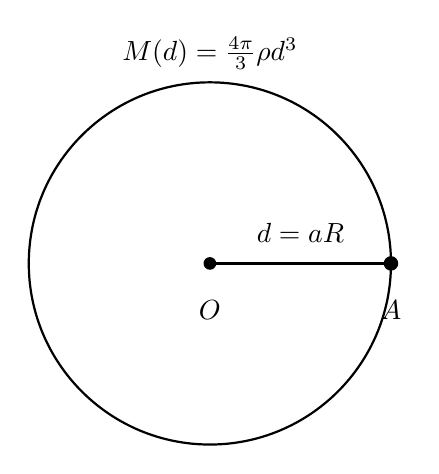
\begin{tikzpicture}[scale=1.15]
\draw[thick] (0,0) circle (2);
\fill (0,0) circle (0.07);
\fill (2,0) circle (0.08);
\draw[thick] (0,0) -- (2,0);
\draw (1,0.12) node[above] {\(d=aR\)};
\draw (0,-0.3) node[below] {\(O\)};
\draw (2,-0.3) node[below] {\(A\)};
\draw (0,2.32) node {\(M(d)=\frac{4\pi}{3}\rho d^3\)};
\end{tikzpicture}
\caption{Ньютоновское упрощение. Для ускорения галактики \(A\) внешние оболочки компенсируются, а масса внутри радиуса \(d\) действует так, как если бы она была сосредоточена в \(O\).}
\label{fig:c01-newton-sphere}
\end{figure}

Для сферически-симметричного распределения массы результирующая сила от вещества вне сферы, проходящей через \(A\), исчезает. Вещество внутри действует так, как если бы оно было сосредоточено в центре. Заключенная масса равна
\begin{equation}
M(d)=\frac{4\pi}{3}\rho d^3.
\label{eq:c01-enclosed-mass}
\end{equation}
Тогда закон Ньютона об обратных квадратах дает ускорение \(A\):
\begin{equation}
\ddot d=-\frac{GM(d)}{d^2}.
\end{equation}
Используя уравнение~\eqref{eq:c01-radial-kinematics},
\begin{align}
\ddot a R
&=-\frac{G}{d^2}\left(\frac{4\pi}{3}\rho d^3\right) \\
&=-\frac{4\pi G}{3}\rho d \\
&=-\frac{4\pi G}{3}\rho aR.
\end{align}
Сопутствующий радиус сокращается, и остается
\begin{equation}
\boxed{\frac{\ddot a}{a}=-\frac{4\pi G}{3}\rho.}
\label{eq:c01-acceleration}
\end{equation}
Это сокращение и есть проверка на согласованность. Каждая галактика, фиксированная в сопутствующих координатах, независимо от \(R\), подчиняется одному и тому же уравнению для одного и того же масштабного фактора.

Подстановка уравнения~\eqref{eq:c01-density-dilution} дает две эквивалентные формы
\begin{equation}
\frac{\ddot a}{a}=-\frac{4\pi G\nu}{3a^3},
\qquad
\ddot a=-\frac{4\pi G\nu}{3a^2}.
\label{eq:c01-acceleration-nu}
\end{equation}
Первая форма показывает относительное ускорение; вторая выделяет \(\ddot a\). Оставлять \(a\) слева — это соглашение, а не изменение физики.

\begin{classroomqa}
\audiencequestion{Начало координат было произвольным, однако каждая сила в вычислении направлена к нему. Как может другой выбор начала координат давать ту же Вселенную?}
\lecturerresponse{Уравнение относится к относительному движению. Повторение вычисления относительно любой другой галактики дает то же самое уравнение, потому что однородность делает заключенную массу зависящей только от физического радиуса. Если перейти к ускоряющейся системе отсчета, связанной с другой галактикой, сохранив при этом силы, отнесенные к первому началу координат, то нужно также включить соответствующую инерциальную силу. Выбор центральной системы покоя лишь избавляет от этого дополнительного учета. Инвариантный результат — это уравнение~\eqref{eq:c01-acceleration}, а не выделенный центр. \lecturetimestamp{00:43:56--00:46:58}}
\end{classroomqa}

\begin{classroomqa}
\audiencequestion{Сохранился бы результат, если бы сопутствующая плотность массы \(\nu\) менялась от места к месту?}
\lecturerresponse{Нет, не в такой форме с одной функцией. Чистое сокращение зависит от \(M\propto d^3\) с одной и той же константой пропорциональности повсюду. Если бы \(\nu\) заметно менялась на масштабе усреднения, разные области потребовали бы разной локальной динамики, и единый однородный масштабный фактор больше не описывал бы их. Однородность здесь играет существенную роль. \lecturetimestamp{00:47:05--00:47:51}}
\end{classroomqa}

\begin{classroomqa}
\audiencequestion{Почему писать \(\ddot a/a\), а не перенести множитель \(a\) вправо?}
\lecturerresponse{Обе формы правильны. В космологии по соглашению пишут относительное ускорение \(\ddot a/a\), отчасти потому, что его можно непосредственно сравнить с относительной скоростью расширения \(H=\dot a/a\). Умножение на \(a\) дает тождественное дифференциальное уравнение. \lecturetimestamp{00:50:36--00:51:29}}
\end{classroomqa}

Уравнение~\eqref{eq:c01-acceleration} немедленно исключает статическую однородную ньютоновскую Вселенную, заполненную обычным веществом. Для статического масштабного фактора было бы \(\ddot a=0\), тогда как положительная плотность делает правую часть отрицательной. Это еще \emph{не} говорит нам, расширяется Вселенная или сжимается. Оно говорит лишь о знаке ускорения.

\section{Отрицательное ускорение — не сжатие}

Различие между скоростью и ускорением элементарно, но решающе. Ferrari, едущая вперед по автобану, может иметь положительную скорость, тормозя при отрицательном ускорении. Точно так же для Вселенной может выполняться
\begin{equation}
\dot a>0,
\qquad
\ddot a<0:
\end{equation}
она расширяется, но расширение замедляется.

Чтобы решить, обращается ли движение в конце концов вспять, сравним космологическую задачу с пробной частицей, движущейся радиально в гравитационном поле Земли. Пусть теперь \(x\) обозначает физическое расстояние частицы от центральной массы \(M\); оно не связано с прежней сопутствующей координатой. Уравнение Ньютона имеет вид
\begin{equation}
\ddot x=-\frac{GM}{x^2}.
\label{eq:c01-particle-force}
\end{equation}
Ускорение всегда направлено внутрь. Частица, брошенная наружу, тем не менее может продолжать двигаться наружу очень долго или вечно. У частицы, уже движущейся внутрь, скорость становится все более отрицательной. Один лишь закон силы не решает, какое движение реализуется; это определяют начальные условия.

\begin{classroomqa}
\audiencequestion{Означает ли \(\ddot a<0\), что Вселенная сжимается?}
\lecturerresponse{Нет. Сжатие означает \(\dot a<0\). Отрицательное \(\ddot a\) означает лишь, что \(\dot a\) уменьшается со временем. Если \(\dot a\) изначально положительно, гравитация замедляет расширение; достигнет ли оно нуля, зависит от начальной скорости расширения, точно так же как судьба тела, движущегося наружу, зависит от того, меньше или больше его скорость скорости убегания. \lecturetimestamp{00:51:30--00:56:18}}
\end{classroomqa}

\begin{figure}[ht]
\centering
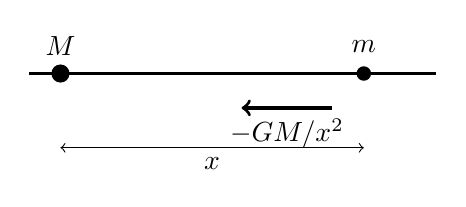
\begin{tikzpicture}[scale=1.15]
\fill (0,0) circle (0.1);
\draw (0,0.3) node {\(M\)};
\draw[thick] (-0.35,0) -- (4.15,0);
\fill (3.35,0) circle (0.08);
\draw (3.35,0.3) node {\(m\)};
\draw[->,very thick] (3.0,-0.38) -- (2.0,-0.38)
  node[midway,below] {\(-GM/x^2\)};
\draw[<->] (0,-0.82) -- (3.35,-0.82)
  node[midway,below] {\(x\)};
\end{tikzpicture}
\caption{Радиальная задача об одной частице, используемая для того, чтобы отделить знак ускорения от направления и дальнейшей судьбы движения.}
\label{fig:c01-particle-sketch}
\end{figure}

Энергия делает альтернативы наглядными. Сохраняющаяся механическая энергия равна
\begin{equation}
E=\frac12 m\dot x^{\,2}-\frac{GMm}{x}.
\label{eq:c01-particle-energy}
\end{equation}
Потенциальная энергия пропорциональна \(1/x\), а не \(1/x^2\); дифференцирование \(-GMm/x\) дает силу, обратно пропорциональную квадрату расстояния.

\begin{figure}[ht]
\centering
\includegraphics[width=0.82\textwidth]{lecture_01_figure_02.png}
\caption{Доска в начале энергетического рассуждения: движущаяся пробная масса и ее кинетический член непосредственно перед тем, как снова вводится гравитационная потенциальная энергия.}
\lectureframe{00:58:57}
\end{figure}

Если \(E<0\), частица, движущаяся наружу, не может достичь бесконечности, где ее потенциальная энергия стремится к нулю, а кинетическая энергия неотрицательна. Она должна остановиться при конечном \(x\) и вернуться. Если \(E>0\), она не может остановиться, потому что в точке поворота кинетическая энергия исчезла бы, а оставшаяся потенциальная энергия была бы отрицательной, что противоречит сохранению положительного \(E\). Граница задается условием
\begin{equation}
E=0,
\end{equation}
которое определяет скорость убегания:
\begin{equation}
\frac12 m v_{\rm esc}^2-\frac{GMm}{x}=0,
\qquad
\boxed{v_{\rm esc}^2=\frac{2GM}{x}.}
\label{eq:c01-escape-velocity}
\end{equation}

\begin{figure}[ht]
\centering
\includegraphics[width=0.88\textwidth]{lecture_01_figure_03.png}
\caption{На доске вырисовывается граница нулевой энергии. Слева прежние космологические уравнения ускорения остаются в рамке, тогда как справа разворачивается радиальная задача об убегании.}
\lectureframe{01:01:37}
\end{figure}

Точно при скорости убегания частица замедляется бесконечно долго. Ее скорость стремится к нулю только при \(x\to\infty\); конечной точки поворота она никогда не достигает. Этот предельный случай станет простейшей космологической моделью.

\section{Космологическое уравнение энергии}

Вернемся к галактике на фиксированном сопутствующем радиусе \(R\). Согласно теореме о сферических оболочках, ее радиальное движение тождественно движению частицы вне точечной массы, равной массе, заключенной внутри ее сопутствующей сферы.

\begin{figure}[ht]
\centering
\includegraphics[width=0.82\textwidth]{lecture_01_figure_04.png}
\caption{Схема силы, обратно пропорциональной квадрату расстояния, и радиальной частицы, используемая при переносе рассуждения об энергии одной частицы обратно в космологию.}
\lectureframe{01:04:14}
\end{figure}

Заключенная масса не возрастает по мере расширения физической сферы. Сфера является сопутствующей, поэтому она всегда содержит одни и те же галактики:
\begin{align}
M
&=\frac{4\pi}{3}\rho(aR)^3 \\
&=\frac{4\pi}{3}\frac{\nu}{a^3}a^3R^3 \\
&=\frac{4\pi}{3}\nu R^3.
\label{eq:c01-fixed-enclosed-mass}
\end{align}
Первое выражение кажется зависящим от времени лишь до тех пор, пока не учтено разрежение плотности. Множители \(a^3\) сокращаются.

\begin{classroomqa}
\audiencequestion{По мере расширения сферы заключает ли она в себе больше массы?}
\lecturerresponse{Нет. Ее физический радиус растет, но ее граница в сопутствующих координатах движется вместе с галактиками. В идеальном однородном потоке никакая материя не пересекает эту границу, и уравнение~\eqref{eq:c01-fixed-enclosed-mass} явно показывает эту компенсацию. \lecturetimestamp{01:04:37--01:05:20}}
\end{classroomqa}

Физическая скорость галактики равна \(\dot d=\dot a R\), а ее расстояние до выбранного начала координат равно \(d=aR\). Следовательно, ее сохраняющаяся ньютоновская энергия равна
\begin{equation}
\boxed{
E=\frac12 m\dot a^{\,2}R^2-\frac{GMm}{aR}.
}
\label{eq:c01-cosmological-energy}
\end{equation}

\begin{figure}[ht]
\centering
\includegraphics[width=0.82\textwidth]{lecture_01_figure_05.png}
\caption{Космологические кинетический и потенциальный члены на доске. Полный знаменатель \(aR\) в уравнении~\eqref{eq:c01-cosmological-energy} получается из физического радиуса и сопровождающего вывода.}
\lectureframe{01:06:12}
\end{figure}

Три случая для энергии частицы переходят в три космологических случая:
\begin{description}[style=nextline]
\item[\(E<0\):] начальное расширение ниже скорости убегания; \(a(t)\) достигает максимума, и вселенная снова коллапсирует.
\item[\(E=0\):] вселенная в точности критическая; расширение замедляется вечно и лишь асимптотически приближается к нулевой скорости.
\item[\(E>0\):] начальное расширение выше скорости убегания; в ньютоновской модели вселенная расширяется вечно с ненулевой асимптотической скоростью разбегания.
\end{description}

Начнем с граничного случая \(E=0\). Приравнивая уравнение~\eqref{eq:c01-cosmological-energy} к нулю, сокращая \(m\) и деля на \(a^2R^2/2\), получаем
\begin{align}
\frac12\dot a^{\,2}R^2&=\frac{GM}{aR}, \\
\left(\frac{\dot a}{a}\right)^2&=\frac{2GM}{a^3R^3}.
\label{eq:c01-energy-intermediate}
\end{align}
Поскольку
\begin{equation}
\rho=\frac{M}{(4\pi/3)a^3R^3},
\end{equation}
уравнение~\eqref{eq:c01-energy-intermediate} принимает вид
\begin{equation}
\boxed{
H^2=\left(\frac{\dot a}{a}\right)^2=\frac{8\pi G}{3}\rho.
}
\label{eq:c01-first-friedmann}
\end{equation}
Это первое уравнение Фридмана для пространственно плоской вселенной, заполненной только веществом, с нулевой космологической постоянной, полученное здесь из ньютоновского закона сохранения энергии.

\begin{classroomqa}
\classquestion{Что происходит с частицей, запущенной точно со скоростью убегания?}
\lecturerresponse{Она замедляется, так и не разворачиваясь. Ее скорость стремится к нулю только на бесконечном расстоянии. Вселенная с нулевой энергией ведет себя так же: \(H\) уменьшается, но величина \(\dot a\) остается положительной, и никакого разворота за конечное время не происходит. \lecturetimestamp{01:10:45--01:12:10}}
\end{classroomqa}

Множители \(4\pi/3\) и \(8\pi G/3\) не являются произвольным украшением. Член \(4\pi/3\) — это объем сферы, а множитель 2 возникает из кинетической энергии. В общей теории относительности тот же \(8\pi G\) входит в уравнение поля Эйнштейна, и его временная-временная компонента приводит к релятивистскому уравнению Фридмана. Это совпадение не случайно, но в данный вывод пока не входят давление, пространственная кривизна в геометрическом смысле и космологическая постоянная.

\section{Критическое решение при доминировании вещества}

Используем закон плотности \(\rho=\nu/a^3\) в уравнении~\eqref{eq:c01-first-friedmann}:
\begin{equation}
\left(\frac{\dot a}{a}\right)^2=\frac{8\pi G\nu}{3a^3}.
\label{eq:c01-matter-friedmann}
\end{equation}
Константа \(\nu\) зависит от произвольной нормировки сопутствующих координат. Чтобы явно выделить зависимость от времени, определим
\begin{equation}
K\equiv\frac{8\pi G\nu}{3}>0.
\end{equation}
Тогда
\begin{equation}
\dot a^{\,2}=\frac{K}{a}.
\label{eq:c01-normalized-friedmann}
\end{equation}

\begin{figure}[ht]
\centering
\includegraphics[width=0.76\textwidth]{lecture_01_figure_06.png}
\caption{Фридмановское масштабирование при доминировании вещества на доске: сначала с константами, а затем с явно выделенной существенной обратностепенной зависимостью от масштабного фактора.}
\lectureframe{01:14:44}
\end{figure}

Правая часть уравнения~\eqref{eq:c01-normalized-friedmann} положительна при каждом конечном положительном \(a\). Для разворота потребовалось бы \(\dot a=0\), поэтому критическая вселенная никогда не разворачивается. Ее расширение неуклонно становится все более вялым, но никогда не настолько, чтобы остановиться.

Теперь решим уравнение. Можно непосредственно разделить переменные,
\begin{equation}
a^{1/2}\,da=\sqrt{K}\,dt,
\end{equation}
или, следуя лекции, попробовать степенной закон,
\begin{equation}
a(t)=Ct^p.
\label{eq:c01-power-trial}
\end{equation}
Тогда
\begin{equation}
\frac{\dot a}{a}=\frac{p}{t},
\qquad
\frac{K}{a^3}=\frac{K}{C^3t^{3p}}.
\end{equation}
Подстановка в уравнение~\eqref{eq:c01-matter-friedmann} дает
\begin{equation}
\frac{p^2}{t^2}=\frac{K}{C^3t^{3p}}.
\end{equation}
Сопоставление степеней и коэффициентов дает
\begin{equation}
3p=2,
\qquad
C^3=\frac{K}{p^2}=\frac{9K}{4}.
\end{equation}
Следовательно,
\begin{equation}
\boxed{
a(t)=\left(\frac{3\sqrt K}{2}t\right)^{2/3}\propto t^{2/3}.
}
\label{eq:c01-two-thirds}
\end{equation}
Начало отсчета времени выбрано так, что \(a=0\) при \(t=0\). В более общем виде можно заменить \(t\) на \(t-t_0\).

Масштабный фактор растет вечно, тогда как
\begin{equation}
\dot a\propto t^{-1/3}\longrightarrow0,
\qquad
H=\frac{2}{3t}\longrightarrow0.
\label{eq:c01-asymptotic-slope}
\end{equation}
Его график всюду возрастает и всюду вогнут вниз. Он не приближается ни к какой горизонтальной прямой, поскольку сам \(a(t)\) неограничен, но его наклон стремится к нулю.

\begin{classroomqa}
\audiencequestion{Форма \(t^{2/3}\) была найдена только потому, что этот пробный вид случайно сработал? Может ли другая пробная форма дать другое решение при нулевой энергии?}
\lecturerresponse{Пробная форма определяет решение, а не просто один из возможных вариантов. Уравнение первого порядка для ветви расширения \(\dot a=\sqrt{K/a}\) интегрируется единственным образом, с точностью до нормировки и выбора начала отсчета времени, в \(a\propto(t-t_0)^{2/3}\). Разным значениям полной энергии соответствуют разные дифференциальные уравнения и, следовательно, разные космологические истории. \lecturetimestamp{01:27:07--01:27:43}}
\end{classroomqa}

\begin{classroomqa}
\audiencequestion{Становится ли критическая кривая в конце концов горизонтальной?}
\lecturerresponse{Ее наклон стремится к нулю: \(\dot a\propto t^{-1/3}\). Тем не менее скорость роста положительна при любом конечном времени, так что масштабный фактор продолжает расти неограниченно. Вселенная асимптотически приближается к покою, не достигая его. \lecturetimestamp{01:27:48--01:28:57}}
\end{classroomqa}

Этот простой результат примечателен в историческом отношении. Ньютон располагал механикой и теоремой о сферической оболочке, необходимыми для этого вывода, и рассматривал вопросы о бесконечной гравитирующей вселенной, но не сформулировал расширяющуюся модель. В обсуждении на занятии было высказано предположение, что философские и теологические убеждения относительно космической истории могли повлиять на то, какие вопросы казались ему естественными. Это историческое предположение не является частью вывода; математическая суть лишь в том, что необходимые ньютоновские инструменты уже существовали.

\begin{classroomqa}
\audiencequestion{Предполагает ли эта ньютоновская конструкция бесконечную вселенную?}
\lecturerresponse{Она предполагает евклидово, пространственно плоское ньютоновское пространство. В обычной ньютоновской модели это пространство простирается неограниченно, так что модель пространственно бесконечна, хотя расстояния между сопутствующими галактиками меняются со временем. Искривленные конечные пространственные геометрии относятся к релятивистскому рассмотрению. \lecturetimestamp{01:22:12--01:22:55}}
\end{classroomqa}

\section{За пределами модели с нулевой энергией}

Случай нулевой энергии — намеренное упрощение, а не единственная ньютоновская вселенная. Если сохранить \(E\neq0\) в уравнении~\eqref{eq:c01-cosmological-energy}, получим
\begin{equation}
\left(\frac{\dot a}{a}\right)^2
=\frac{8\pi G}{3}\rho+\frac{2E}{mR^2a^2}.
\label{eq:c01-nonzero-energy}
\end{equation}
Однородность требует, чтобы комбинация \(2E/(mR^2)\) была одной и той же для любой представительной сопутствующей сферы. Обозначая ее константой \(C_E\),
\begin{equation}
H^2=\frac{8\pi G}{3}\rho+\frac{C_E}{a^2}.
\end{equation}
Положительное \(C_E\) соответствует энергии, превышающей энергию убегания; отрицательное \(C_E\) допускает разворот. В релятивистских обозначениях этот энергетический член переинтерпретируется через пространственную кривизну; эта связь оставлена для дальнейшего рассмотрения.

Все три истории в модели только с веществом имеют отрицательное ускорение, пока доминирует вещество:
\begin{equation}
\ddot a=-\frac{4\pi G}{3}\rho a<0.
\end{equation}
Кривая с повторным коллапсом растет, достигает точки, где \(\dot a=0\), и затем падает. Критическая кривая \(t^{2/3}\) растет вечно, причем ее наклон стремится к нулю. Кривая положительной энергии тоже растет вечно и приближается к линейному росту. Предварительный набросок этих случаев на доске был исправлен по ходу лекции; устойчивый вывод состоит в их общей вогнутости вниз, а не в каждой детали первого эскиза.

Наблюдаемая вселенная ведет себя сложнее. Ее раннее расширение при доминировании вещества хорошо аппроксимируется замедляющейся кривой, но на поздних временах кривая изгибается вверх:
\begin{equation}
\ddot a>0.
\end{equation}
Обычное вещество без давления не может дать такой знак в уравнении~\eqref{eq:c01-acceleration}. Требуется дополнительный член. В простейшей современной модели это космологическая постоянная; более общо это называют темной энергией. Данная глава намеренно его опускает, чтобы сначала можно было в чистом виде понять ньютоновскую динамику вещества.

\begin{classroomqa}
\audiencequestion{Является ли \(8\pi G\) в уравнении Фридмана тем же множителем, который появляется в уравнении поля Эйнштейна, и включили ли мы космологическую постоянную?}
\lecturerresponse{Тот же гравитационный нормировочный множитель появляется в общей теории относительности, и временная-временная компонента уравнения поля воспроизводит релятивистское уравнение Фридмана. Модель здесь не содержит космологической постоянной. Это вселенная, доминированная веществом; отсутствующий член с космологической постоянной как раз и является тем типом члена, который может объяснить позднее ускорение. \lecturetimestamp{01:30:15--01:31:06}}
\end{classroomqa}

\section{Средний поток и локальные отклонения}

Однородное расширение — это крупнозернистое описание. Оно не утверждает, что каждый объект удаляется от каждого ближайшего соседа. Гравитационно или иным образом связанные системы могут выйти из хаббловского потока. Млечный Путь и Андромеда, например, сближаются друг с другом, а не следуют крупномасштабному закону разбегания.

Отклонение скорости отдельной галактики от хаббловского потока называется ее \emph{пекулярной скоростью}. Этот термин технический, а не оценка галактики. Закон Хаббла становится лучшим приближением при усреднении по большим расстояниям и большим объемам. На масштабе галактики как связанной системы, скопления или локально переуплотненной области локальные силы могут преобладать над фоновым расширением.

\begin{classroomqa}
\audiencequestion{Могут ли некоторые области сжиматься, хотя Вселенная в целом расширяется?}
\lecturerresponse{Конечно. Связанные системы и достаточно плотные флуктуации не обязаны следовать среднему расширению. Система Млечного Пути--Андромеды — хорошо известный пример. В космологическом расчёте усреднение ведётся по настолько большим объёмам, что эти пекулярные движения и локальные флуктуации плотности не доминируют; тогда \(a(t)\), полученное таким образом, описывает фон, а не каждую пару объектов. \lecturetimestamp{01:31:00--01:34:13}}
\end{classroomqa}

В качестве аналогии можно взять обычный газ. Когда воздух в комнате называют однородным, этим не отрицают молекулярные флуктуации или локальные вариации плотности. Это означает, что средние по достаточно большим областям устойчивы. Космическая однородность имеет тот же логический статус, хотя и на несравненно больших масштабах. Область, возникшая с плотностью немного выше средней, может обладать достаточной самогравитацией, чтобы сопротивляться расширению и в конечном счёте коллапсировать в связанную структуру.

\begin{classroomqa}
\audiencequestion{Могут ли наблюдения решить, движутся ли галактики в пространстве или же расширение пространства раздвигает их друг от друга?}
\lecturerresponse{Нет, если в обоих описаниях каждой паре приписывается одно и то же расстояние \(d_{AB}(t)\). В одном описании галактики движутся на координатном фоне, который выглядит фиксированным; в сопутствующей картине они остаются на месте, а изменение берёт на себя масштабный фактор. Обе картины математически эквивалентны. Общая теория относительности делает такой язык описания более естественным, но в этом сравнении не создаёт отдельной наблюдаемой величины. \lecturetimestamp{01:34:14--01:34:59}}
\end{classroomqa}

\begin{classroomqa}
\audiencequestion{Помимо яркости сверхновых типа Ia, есть ли независимые свидетельства космического ускорения?}
\lecturerresponse{Да. Такой вывод опирается на совокупность наблюдений, особенно на то, как согласуются между собой измерения сверхновых и космического микроволнового фона. Он не опирается на одну-единственную точку данных; важно согласие между независимыми космологическими измерениями. \lecturetimestamp{01:35:00--01:35:38}}
\end{classroomqa}

\section{Что было установлено}

Рассуждение шло в строгом порядке:
\begin{enumerate}
\item Крупномасштабная изотропия вместе с отказом от выделенного центра делает естественной однородность.
\item Однородность допускает сопутствующую координатную сетку с одним масштабным фактором \(a(t)\).
\item Дифференцируя физическое расстояние, получаем закон Хаббла,
  \[
  H=\frac{\dot a}{a},
  \qquad
  v=Hd.
  \]
\item Из сохранения массы в сопутствующей ячейке следует
  \[
  \rho=\frac{\nu}{a^3}.
  \]
\item Из теоремы Ньютона об оболочке следует уравнение ускорения
  \[
  \frac{\ddot a}{a}=-\frac{4\pi G}{3}\rho.
  \]
\item Сохранение энергии позволяет различать расширение с повторным коллапсом, критическое и неограниченное.
\item При нулевой полной энергии,
  \[
  H^2=\frac{8\pi G}{3}\rho,
  \qquad
  a(t)\propto t^{2/3}.
  \]
\end{enumerate}

Это полная ньютоновская модель с доминированием вещества, но ещё не полное описание нашей Вселенной. Она отражает раннюю логику замедляющегося расширения, показывает, почему заполненная однородная Вселенная не может оставаться статической, и выделяет критическое расширение на пороге убегания. Остаётся добавить ненулевую энергию, релятивистскую пространственную геометрию, давление, излучение и член, ответственный за позднее ускорение.
